\documentclass[xcolor=dvipsnames,aspectratio=159]{beamer}
\usetheme{SimpleDarkBlue}

\usepackage{hyperref}
\usepackage{graphicx}
\usepackage{booktabs}
\usepackage[spanish]{babel}
\usepackage[utf8]{inputenc}
\usepackage{amsmath}
\usepackage{amssymb}
\usepackage{amsthm}
\usepackage{graphics}
\usepackage{subfigure}
\usepackage{lipsum}
\usepackage{array}
\usepackage{multicol}
\usepackage{enumerate}
\usepackage[framemethod=TikZ]{mdframed}
\usepackage{geometry}
\usepackage{tikz}
\usepackage{pgffor}
\usepackage{ifthen}
\usepackage{enumitem}
\usepackage{hyperref}
\usepackage{listings}
\usepackage{bbm}
\usepackage{nopageno}

%Gestión de Hipervínculos

\hypersetup{
    colorlinks=true,
    linkcolor=black,
    filecolor=magenta,      
    urlcolor=cyan
}

%En esta parte se hacen redefiniciones de algunos comandos para que resulte agradable el verlos%

\def\proof{Demostración:\\}
\def\endproof{\hfill$\blacksquare$}

\def\sol{Solución:\\}
\def\endsol{\hfill$\square$}

%En esta parte se definen los comandos a usar dentro del documento para enlistar%

\newtheoremstyle{largebreak}
  {}% use the default space above
  {}% use the default space below
  {\normalfont}% body font
  {}% indent (0pt)
  {\bfseries}% header font
  {}% punctuation
  {\newline}% break after header
  {}% header spec

\theoremstyle{largebreak}

\newmdtheoremenv[
    hidealllines = true
]{exa}{Ejemplo}[section]

\newmdtheoremenv[
    hidealllines = true
]{obs}{Observación}[section]

\newmdtheoremenv[
    hidealllines = true
]{theor}{Teorema}[section]

\BeforeBeginEnvironment{theor}{
    \setbeamercolor{block title}{fg=white,bg=red!80!blue}
}

\newmdtheoremenv[
    hidealllines = true
]{propo}{Proposición}[section]

\BeforeBeginEnvironment{propo}{
    \setbeamercolor{block title}{fg=white,bg=blue!80!black}
}

\newmdtheoremenv[
    hidealllines = true
]{cor}{Corolario}[section]

\newmdtheoremenv[
    hidealllines = true
]{lema}{Lema}[section]

\newmdtheoremenv[
    hidealllines = true
]{mydef}{Definición}[section]

\BeforeBeginEnvironment{mydef}{
    \setbeamercolor{block title}{fg=white,bg=gray!80!black}
}

\newmdtheoremenv[
    hidealllines = true
]{excer}{Ejercicio}[section]



%En esta parte se colocan comandos que definen la forma en la que se van a escribir ciertas funciones%

\newcommand\abs[1]{\ensuremath{\left|#1\right|}}
\newcommand\divides{\ensuremath{\bigm|}}
\newcommand\cf[3]{\ensuremath{#1:#2\rightarrow#3}}
\newcommand\contradiction{\ensuremath{\#_c}}
\newcommand\natint[1]{\ensuremath{\left[\big|#1\big|\right]}}
\newcounter{figcount}
\setcounter{figcount}{1}
\newcommand{\bbm}[1]{\ensuremath{\mathbbm{#1}}}
\newcommand{\pint}[2]{\langle#1\big|#2 \rangle}
\newcommand{\norm}[1]{\|#1\|}
\newcommand{\Isom}[1]{\ensuremath{\textup{Isom}\left(#1\right)}}
\newcommand{\SO}[1]{\ensuremath{\textup{SO}\left(#1\right)}}
\newcommand\Aut[1]{\ensuremath{\textup{Aut}\left(#1\right)}}
\newcommand{\Cay}[1]{\ensuremath{\textup{Cay}\left(#1\right)}}
\newcommand{\gen}[1]{\ensuremath{\langle#1\rangle}}
\newcommand{\qisom}{\ensuremath{\underset{C.I.}{\sim}}}
\newcommand{\SL}[1]{\ensuremath{\textup{SL}\left(#1\right)}}
\newcommand{\PSL}[1]{\ensuremath{\textup{PSL}\left(#1\right)}}
\newcommand{\Tr}[1]{\ensuremath{\textup{Tr}\left(#1\right)}}
\newcommand{\im}[1]{\ensuremath{\textup{im}\left(#1\right)}}
\newcommand{\Diam}[1]{\ensuremath{\textup{diam}\left(#1\right)}}
\newcommand{\arcosh}[1]{\ensuremath{\textup{arcosh}\left(#1\right)}}
\newcommand{\centered}[1]{\begin{tabular}{l} #1 \end{tabular}}

%----------------------------------------------------------------------------------------
%    TITLE PAGE
%----------------------------------------------------------------------------------------

\subtitle{Proyecto: Grupos y Geometría: Acciones, Dimensión y Dualidad}
\title{Hiperbolicidad: Ejemplos y Aplicaciones en Teoría Geométrica de Grupos}

\author{Cristo Daniel Alvarado}

\institute
{
    Escuela Superior de Física y Matemáticas \\
    Instituto Politécnico Nacional
}
\date{\today} % Date, can be changed to a custom date

%----------------------------------------------------------------------------------------
%    PRESENTATION SLIDES
%----------------------------------------------------------------------------------------

\begin{document}

\begin{frame}
    \titlepage
\end{frame}

%----------------------------------------------------------------------------------------
\section{Espacios Hiperbólicos}
%----------------------------------------------------------------------------------------

\begin{frame}{Espacios Hiperbólicos}
    \begin{center}
        \LARGE{Espacios Hiperbólicos y el Problema de la Palabra}
    \end{center}

    \pause

    \begin{center}
        Hablaremos de triángulos.
    \end{center}
    \begin{figure}
        \begin{center}
            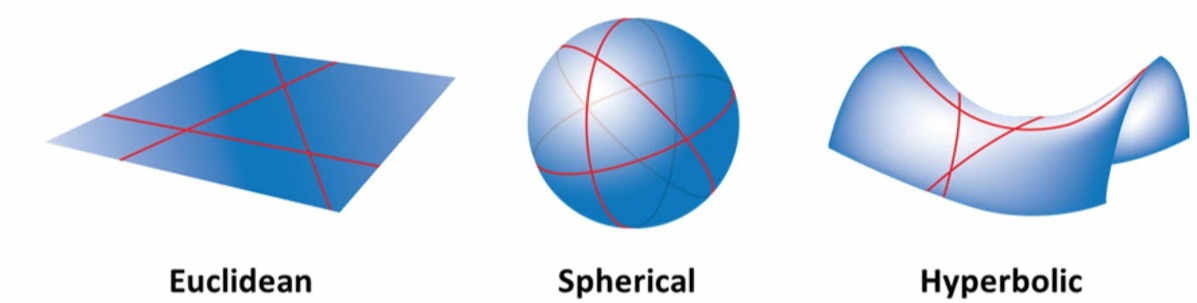
\includegraphics[scale=0.25]{images/all_triangles.png}
        \end{center}
    \end{figure}
    \begin{center}
        y luego de grupos... 
    \end{center}

\end{frame}

\begin{frame}{Hiperbólicidad y $\delta$-hiperbolicidad}
    \begin{center}
        Triángulos geodésicos sobre superficie \textit{hiperbólica}:
    \end{center}
    \begin{figure}
        \begin{center}
            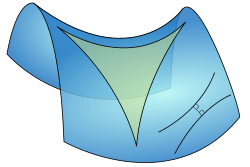
\includegraphics[scale=0.5]{images/hyperbolic_triangle_2.png}
        \end{center}
    \end{figure}
\end{frame}

\begin{frame}{Hiperbólicidad y $\delta$-hiperbolicidad}
    \textbf{Idea}: generalizar noción de hiperbolicidad a espacios métricos.
    \begin{itemize}
        \item Queremos conservar noción de distancia mínima (geodésicas).
        \item Vía triángulos geodésicos.
        \item Ensanchamientos.
    \end{itemize}

    \pause
    \begin{figure}
        \begin{center}
            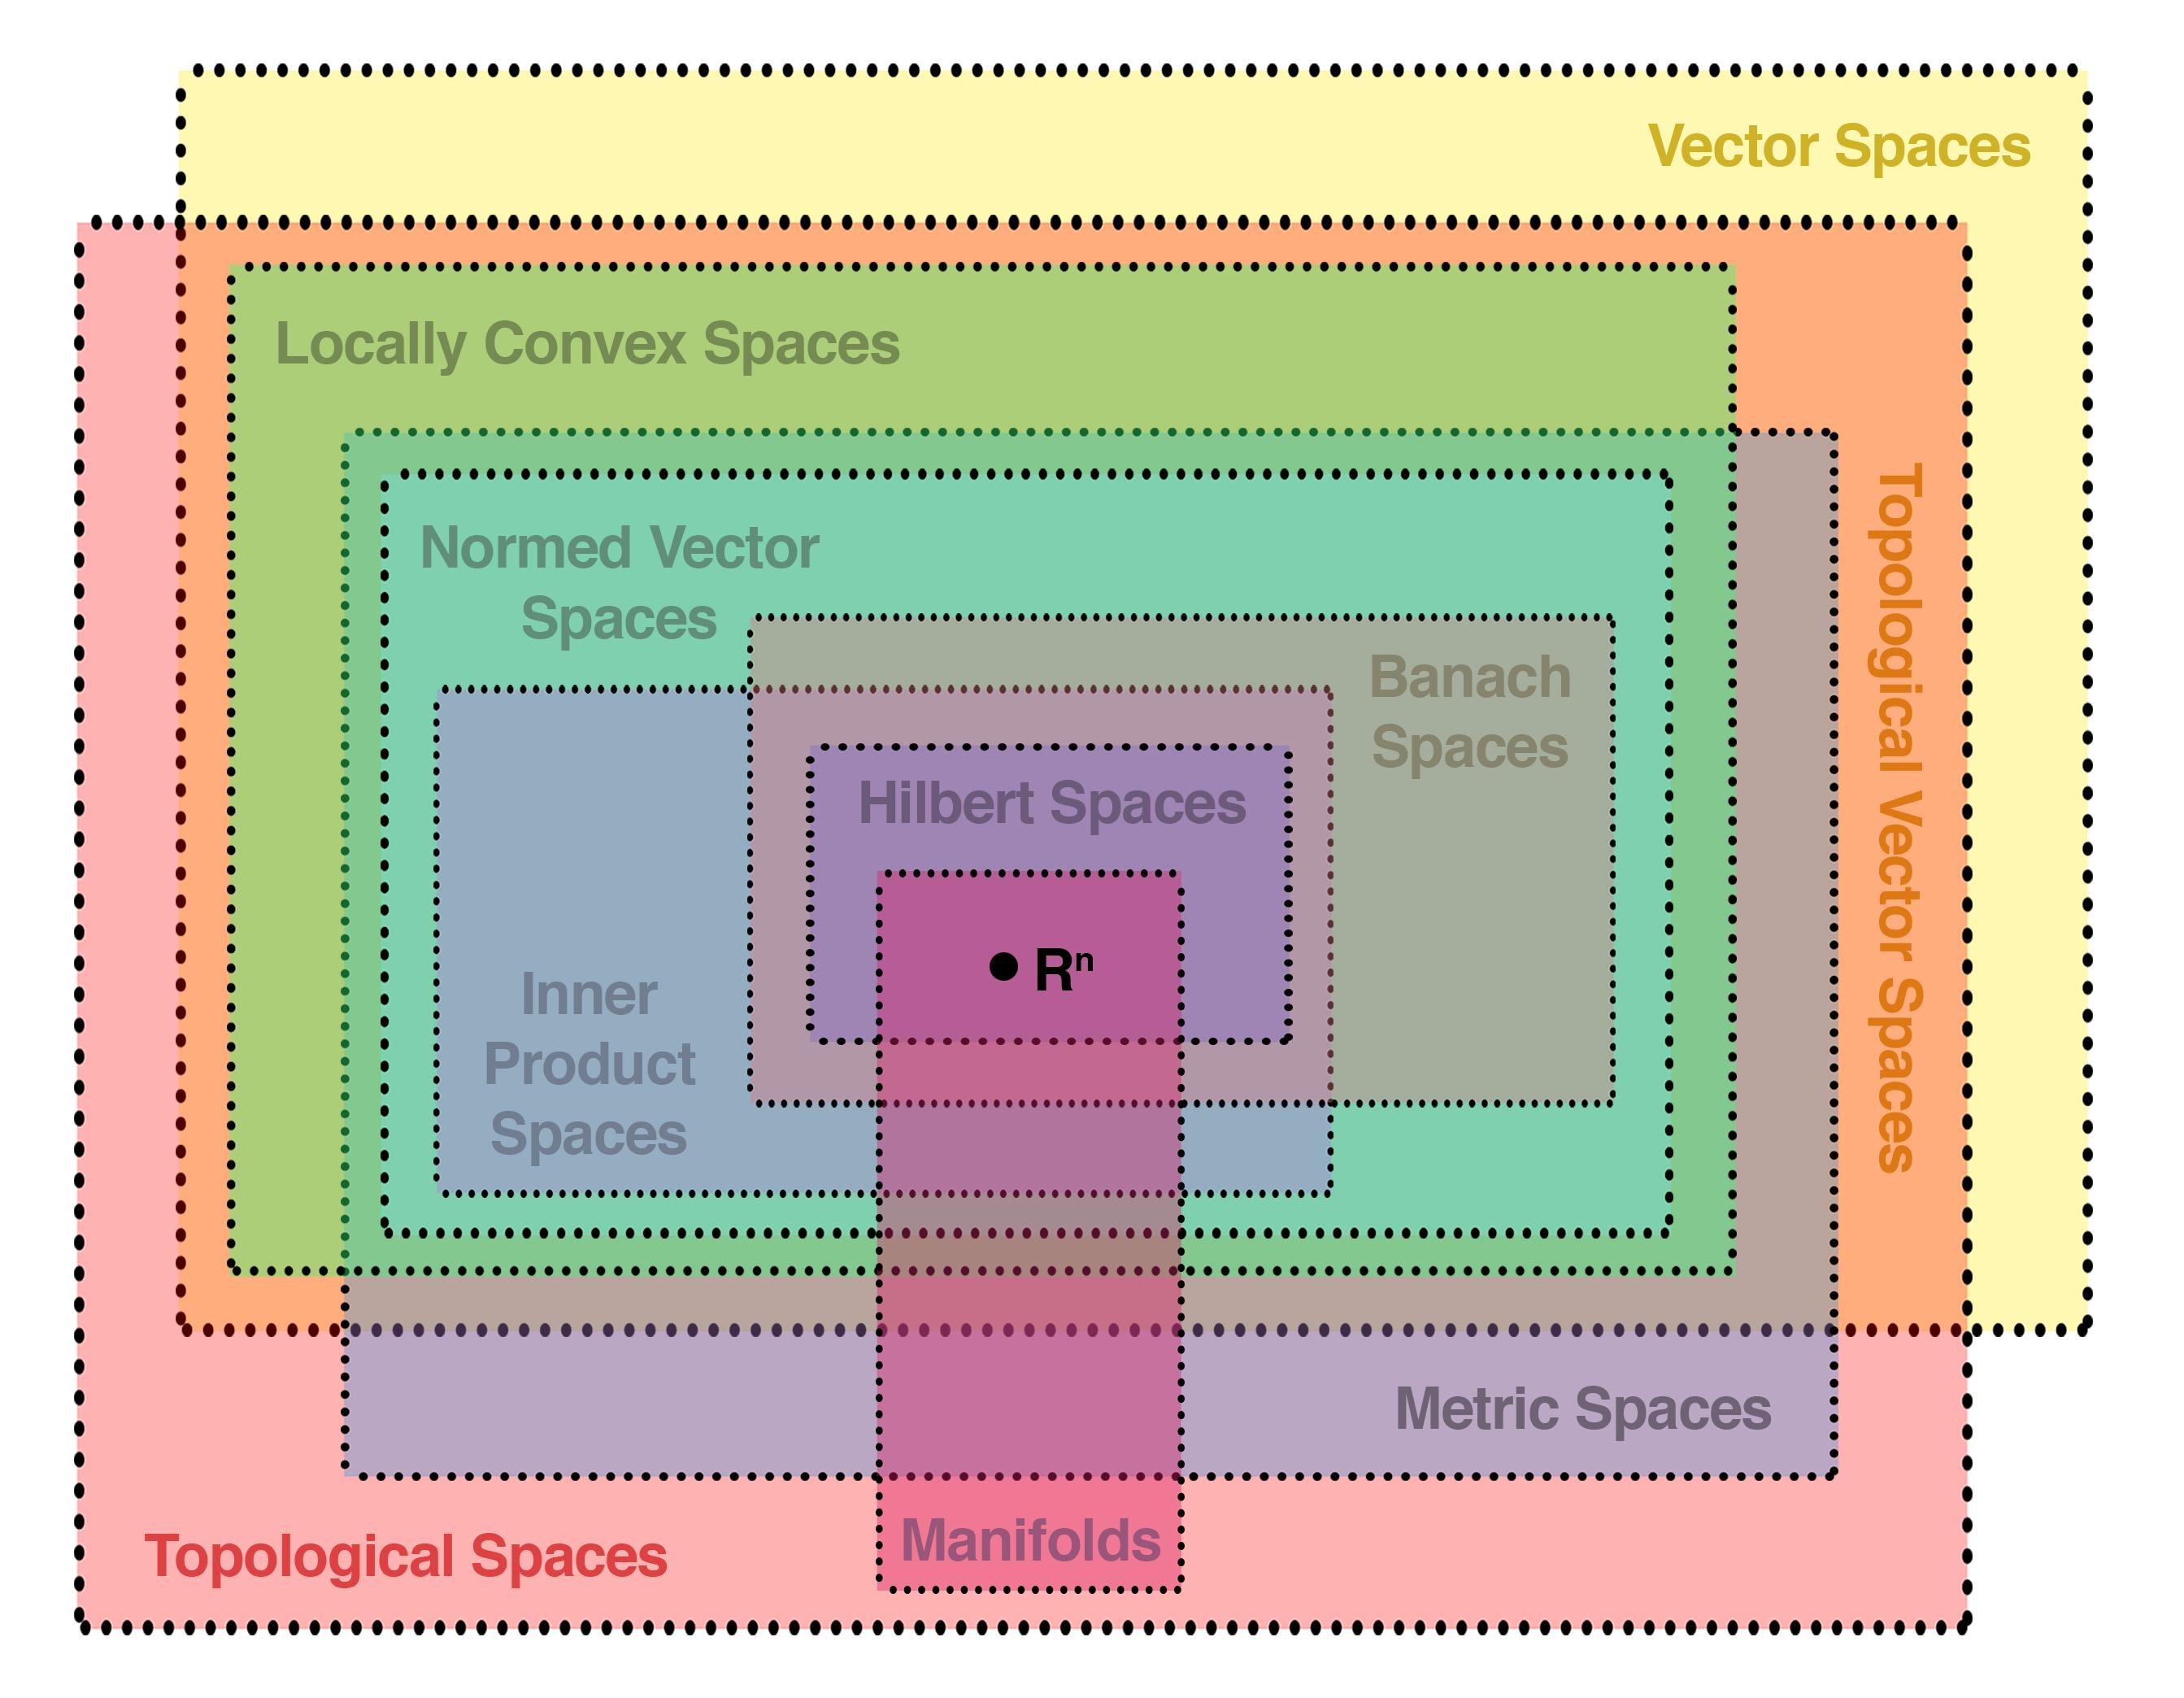
\includegraphics[scale=0.08]{images/hiearchy.jpg}
        \end{center}
    \end{figure}
\end{frame}

\begin{frame}{Hiperbólicidad y $\delta$-hiperbolicidad}
    \begin{center}
        Geodésicas:
    \end{center}
    \begin{figure}
        \begin{center}
            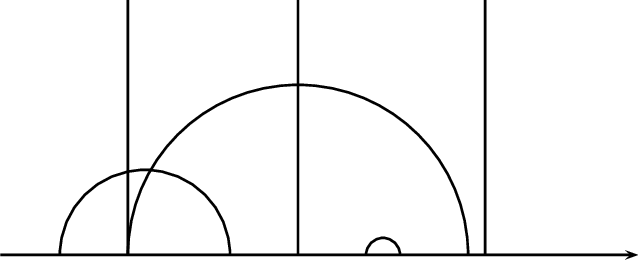
\includegraphics[scale=0.8]{images/geodesics_half_plane.png}
        \end{center}
    \end{figure}
    \pause
    \begin{center}
        Triángulos geodésicos:
    \end{center}
    \begin{figure}
        \begin{center}
            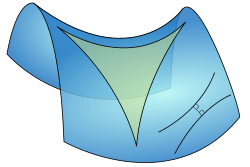
\includegraphics[scale=0.3]{images/hyperbolic_triangle_2.png}
        \end{center}
    \end{figure}
\end{frame}

\begin{frame}{Hiperbólicidad y $\delta$-hiperbolicidad}
    \begin{center}
        Ensanchamiento:
    \end{center}
    \begin{figure}
        \begin{center}
            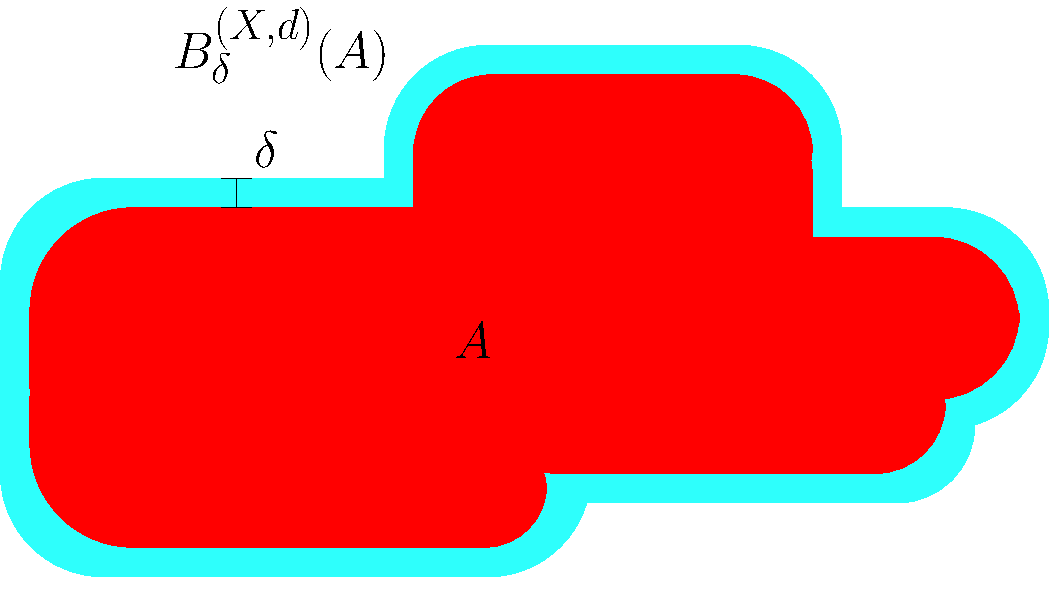
\includegraphics[scale=0.6]{images/B_delta.pdf}
        \end{center}
        \caption{Ejemplo de conjunto $A$ y $B_\delta^{(X,d)}(A)$ (ensanchamiento de $A$).}
    \end{figure}
\end{frame}

\begin{frame}{Hiperbólicidad y $\delta$-hiperbolicidad}
    \begin{mydef}
        Sea $(X,d)$ un espacio métrico. Para cada $\delta>0$ y para cada $A\subseteq X$ se define el conjunto:
        \begin{equation*}
            B_\delta^{(X,d)}(A)=\left\{x\in X\Big|\exists a\in A\textup{ tal que }d(x,a)\leq\delta \right\}
        \end{equation*}
        en este caso $B_\delta^{(X,d)}(A)$ será llamado \textbf{ensanchamiento de $A$ por factor $\delta$}.
    \end{mydef}
\end{frame}

\subsection{Hiperbólicidad y $\delta$-hiperbolicidad}

\begin{frame}{Hiperbólicidad y $\delta$-hiperbolicidad}
    \begin{mydef}[\textbf{Triángulos geodésicos $\delta$-delgados}]
        Sea $(X,d)$ un espacio métrico. Un \textbf{triángulo geodésico en $X$} es una tripleta $(\gamma_0,\gamma_1,\gamma_2)$ de geodésicas $\cf{\gamma_i}{[0,L_i]}{X}$ en $X$ tales que:
        \begin{equation*}
            \gamma_0(L_0)=\gamma_1(0),\quad \gamma_1(L_1)=\gamma_2(0),\quad \gamma_2(L_2)=\gamma_0(0)
        \end{equation*}
    \end{mydef}

    \begin{mydef}[\textbf{Triángulos geodésicos $\delta$-delgados}]
        Un triángulo geodésico es \textbf{$\delta$-delgado} si:
        \begin{equation*}
            \begin{array}{cc}
                \im{\gamma_0}&\subseteq B_{\delta}^{(X,d)}(\im{\gamma_1}\cup\im{\gamma_2}),\\
                \im{\gamma_1}&\subseteq B_{\delta}^{(X,d)}(\im{\gamma_0}\cup\im{\gamma_2}),\\
                \im{\gamma_2}&\subseteq B_{\delta}^{(X,d)}(\im{\gamma_0}\cup\im{\gamma_1})
            \end{array}
        \end{equation*}
    \end{mydef}
\end{frame}

\begin{frame}{Hiperbólicidad y $\delta$-hiperbolicidad}
    \textbf{Noción}: Hacer que los ensanchamientos de dos lados contengan al otro lado.
    \pause    
    \begin{figure}
        \begin{center}
            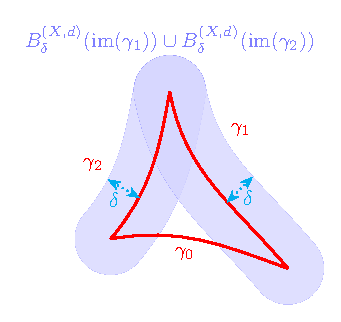
\includegraphics[scale=1.25]{images/delta_slim_2.pdf}
        \end{center}
        \caption{Triángulo geodésico $\Delta=(\gamma_0,\gamma_1,\gamma_2)$ y $B_\delta^{(X,d)}$.}
    \end{figure}
\end{frame}


\begin{frame}{Hiperbólicidad y $\delta$-hiperbolicidad}
    \begin{center}
        \textit{\Large ¿El triángulo anterior es $\delta$-delgado?}
    
        \pause

        \hfill\break

        \Large No, la imagen de $\gamma_0$ no está contenida en $B_\delta^{(X,d)}(\im{\gamma_1})\cup B_\delta^{(X,d)}(\im{\gamma_2})$.
    \end{center}
\end{frame}

\begin{frame}{Hiperbólicidad y $\delta$-hiperbolicidad}
    \begin{mydef}[\textbf{Espacios hiperbólicos}]
        Sea $(X,d)$ un espacio métrico.
        \begin{enumerate}[label = \textit{(\arabic*)}]
            \item Sea $\delta\in\bbm{R}_{\geq0}$. Decimos que $(X,d)$ es \textbf{$\delta$-hiperbólico} si $X$ es geodésico y todos los triángulos geodésicos de $X$ son $\delta$-delgados.
            
            \pause

            \item $(X,d)$ es \textbf{hiperbólico} si existe $\delta\in\bbm{R}_{\geq0}$ tal que $(X,d)$ es $\delta$-hiperbólico.
        \end{enumerate}
    \end{mydef}
\end{frame}

\begin{frame}{Hiperbólicidad y $\delta$-hiperbolicidad}
    \begin{center}
        \Large Ejemplos:
    \end{center}
    \begin{center}
        \begin{tabular}{ c  c  c }
            \centered{\raisebox{-\totalheight}{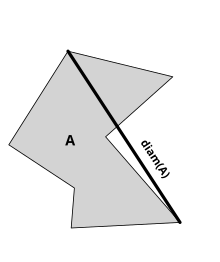
\includegraphics[scale = 0.35]{images/finite_diameter.png}}} & \centered{\raisebox{-\totalheight}{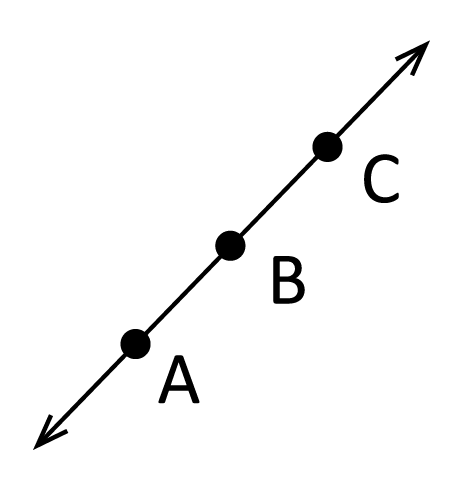
\includegraphics[scale = 0.10]{images/real_line.png}}} & \centered{\raisebox{-\totalheight}{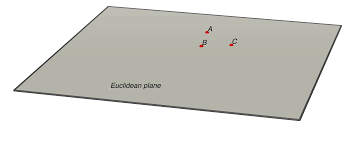
\includegraphics[scale = 0.3]{images/euclidean_plane.png}}} \\
          Espacio de diámetro finito & Recta Real & Plano Euclideano \\
          \pause
            &  &  \\
            \hline
            &  &  \\
          $\Diam{A}$-hiperbólico & $0$-hiperbólico & No es hiperbólico \\
      \end{tabular}
    \end{center}
\end{frame}

\begin{frame}{Hiperbólicidad y $\delta$-hiperbolicidad}
    \begin{center}
        ¿Por qué $\bbm{R}^2$ no es hiperbólico?
    \end{center}
    \pause
    \begin{figure}
        \begin{center}
            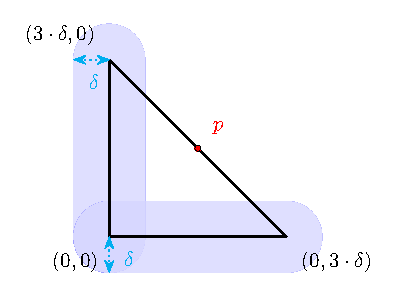
\includegraphics[scale=1.25]{images/hiperbolicnt_euclidean_plane.pdf}
        \end{center}
        \caption{Triángulo que no es $\delta$-hiperbólico.}
    \end{figure}
\end{frame}

\begin{frame}{Hiperbólicidad y $\delta$-hiperbolicidad}
    \begin{center}
        \Large Con esta nueva definición surge una duda:
        
        \pause

        \hfill\break

        \textit{¿Coincide esta nueva noción de hiperbolicidad de espacios métricos con la definición sobre superficies?}
    \end{center}
\end{frame}

\subsection{Hiperbolicidad del Plano $\bbm{H}^2$}

\begin{frame}
    \begin{center}
        \Large Hiperbolicidad del Plano $\bbm{H}^2$...
    \end{center}
    \begin{figure}
        \begin{center}
            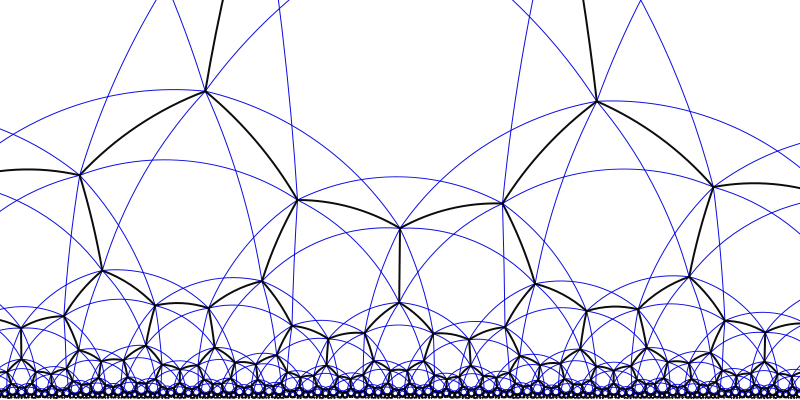
\includegraphics[scale=0.4]{images/hyperbolic_plane.png}
        \end{center}
    \end{figure}

    \pause

    \begin{center}
        como espacio métrico
    \end{center}
    
\end{frame}

\begin{frame}{Hiperbolicidad del Plano $\bbm{H}^2$}
    \begin{mydef}[\textbf{Integral hiperbólica y Área hiperbólica}]
        Si $A\subseteq H$ es un conjunto Lebesgue medible, definimos el \textbf{área hiperbólica de $A$} por:
        \begin{equation*}
            \mu_{\bbm{H}^2}(A)=\int_{H}\chi_A\:dA_{\bbm{H}^2}=\int_{H}\frac{\chi_A}{y^2}\:dxdy
        \end{equation*}
    \end{mydef}

    \pause
    
    \begin{exa}[\textbf{Cuadrado}]
        \begin{columns}
        % Primera columna con la imagen
        \column{0.4\textwidth}
            \centering \includegraphics[width=0.55\linewidth]{images/Cuadrado}
        
        % Segunda columna con la ecuación
        \column{0.4\textwidth}
            \begin{equation*}
                \begin{split}
                    \mu_{\bbm{H}^2}(A) &= \int_{0}^{e^{2/10}} \int_{1}^{e} \frac{dx\,dy}{y^2} \\ 
                    &= e^{\frac{2}{10}} \left(1 - e^{-1} \right)
                \end{split}
            \end{equation*}
        \end{columns}
    \end{exa}    
\end{frame}

\begin{frame}{Hiperbolicidad del Plano $\bbm{H}^2$}
  \begin{columns}
    % Primera columna con el teorema
    \column{0.6\textwidth}
    \begin{theor}[\textbf{Teorema de Gauß-Bonnet para triángulos hiperbólicos}]
      Sea $\Delta$ un triángulo geodésico no degenerado en $(H,d_H)$ con ángulos $\alpha,\beta,\gamma$. Entonces:
      \begin{equation*}
        \mu_{\mathbb{H}^2}(\Delta) = \pi - (\alpha + \beta + \gamma)
      \end{equation*}
      \pause
      En particular:
      \begin{equation*}
        \mu_{\mathbb{H}^2}(\Delta) < \pi
      \end{equation*}
    \end{theor}

    % Segunda columna con la imagen
    \column{0.4\textwidth}
    \begin{figure}
      \centering
      \includegraphics[width=0.8\linewidth]{images/Triangle.png}
    \end{figure}
  \end{columns}
\end{frame}

%Añadir dibujo de B_r y Q_r

\begin{frame}{Hiperbolicidad del Plano $\bbm{H}^2$}
    \begin{propo}[\textbf{Crecimiento exponencial del área hiperbólica}]
        Para todo $r\in\bbm{R}_{>10}$:
        \begin{equation*}
            \mu_{\bbm{H}^2}(B_r^{(H,d_H)}(i))\geq e^{\frac{r}{10}}(1-e^{-\frac{r}{2}})
        \end{equation*}
    \end{propo}
    
  \begin{columns}
    % Primera columna con la demostración
    \column{0.5\textwidth}
    \begin{proof}
      \pause
      Sea $r \in \mathbb{R}_{>10}$, el conjunto:
      \begin{equation*}
        Q_r = \left\{ x + iy \; \Big| \; x \in [0, e^{r/10}], \; y \in [1, e^{r/2}] \right\}
      \end{equation*}
      está contenido en $B_r^{(H, d_H)}(i)$. En particular:
      \pause
      \begin{equation*}
        \begin{split}
          \mu_{\mathbb{H}^2}(B_r^{(H, d_H)}(i)) &\geq \mu_{\mathbb{H}^2}(Q_r) \\
          &= \int_{0}^{e^{r/10}} \int_{1}^{e^{r/2}} \frac{dx\,dy}{y^2} \\
          &= e^{\frac{r}{10}} \left(1 - e^{-\frac{r}{2}} \right)
        \end{split}
      \end{equation*}
    \end{proof}

    % Segunda columna con la imagen
    \column{0.5\textwidth}
    \begin{figure}
      \centering
      \includegraphics[width=0.7\linewidth]{images/Circle.pdf}
    \end{figure}
  \end{columns}
\end{frame}

\begin{frame}{Hiperbolicidad del Plano $\bbm{H}^2$}
    \begin{theor}[\textbf{Triángulos son delgados}]
        Existe una constante $\delta\in\bbm{R}_{\geq0}$ tal que todo triángulo geodésico en $(H,d_H)$ es $\delta$-delgado.
    \end{theor}

    \pause

    \textit{Demostración:}

    Por la proposición anterior, existe $\delta>0$ tal que:
    \begin{equation*}
        \mu_{\bbm{H}^2}(B_\delta^{(H,d_H)}(i))\geq 2\cdot\pi
    \end{equation*}
    \pause
    (por ejemplo $\delta=14$).
    \pause
    Tomemos $\Delta=(\gamma_0,\gamma_1,\gamma_2)$ un triángulo geodésico en $(H,d_H)$ y sea $x\in\im{\gamma_0}$.
\end{frame}

\begin{frame}{Hiperbolicidad del Plano $\bbm{H}^2$}
    \begin{figure}
        \begin{center}
            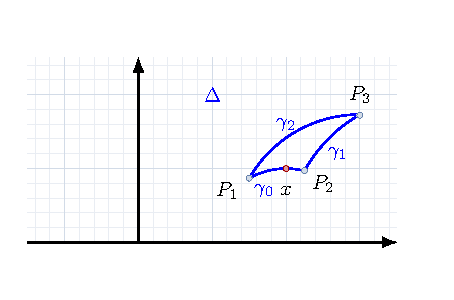
\includegraphics[scale=1]{images/uhp_geodesic_triangle.pdf}
        \end{center}
    \end{figure}
    \pause
    Dos casos:
    \begin{itemize}
        \pause
        \item $\Delta$ es degenerado (está en una línea geodésica). Es inmediato.
        \pause
        \item Trasladamos con una isometría la geodésica de $P_1$ a $P_2$ al eje $y$ tal que $x$ vaya a $i$.
    \end{itemize}
\end{frame}

%TODO: Cambiar imagen para que sea correcta y poner dos imágenes para que se vaya entendiendo el procedimiento.

\begin{frame}{Hiperbolicidad del Plano $\bbm{H}^2$}
    \begin{figure}
        \begin{center}
            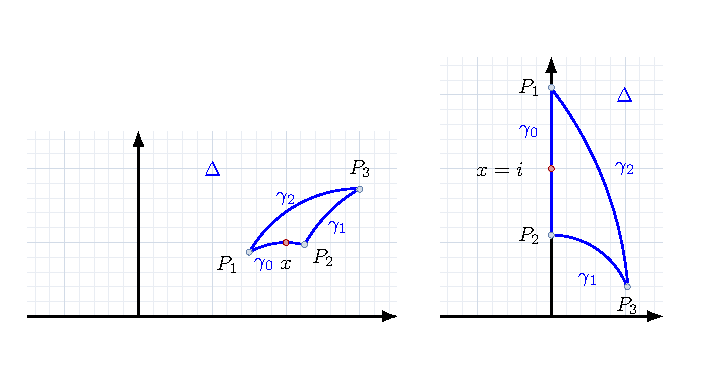
\includegraphics[scale=1]{images/uhp_geodesic_triangle_2.pdf}
        \end{center}
        \caption{Movimiento de $\Delta$ por isometría.}
    \end{figure}
\end{frame}

\begin{frame}{Hiperbolicidad del Plano $\bbm{H}^2$}
    \begin{figure}
        \begin{center}
            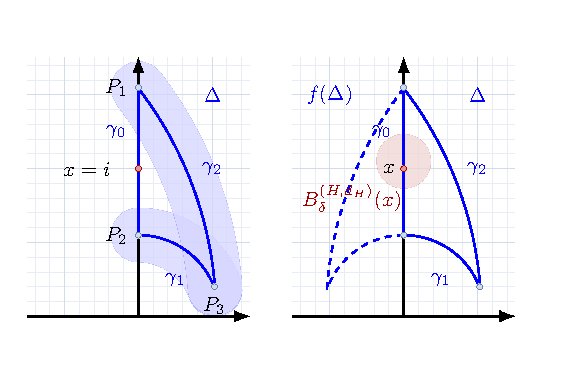
\includegraphics[scale=1]{images/uhd_geodesic_triangle_4.pdf}
        \end{center}
        \caption{Ensanchamiento de los lados $\gamma_1$ y $\gamma_2$, junto con la bola centrada en $i$ de radio $\delta$ y la reflexión de $\Delta$.}
    \end{figure}
\end{frame}


\begin{frame}{Hiperbolicidad del Plano $\bbm{H}^2$}
    Supongamos $\forall y\in\im{\gamma_1}\cup\im{\gamma_2}$, $d_H(x,y)>C$. Se tiene entonces que:
    \begin{equation*}
        B_c^{(H,d_H)}(i)\subseteq \Delta\cup\im{\gamma_0}\cup f(\Delta)
    \end{equation*}
    \pause
    con $\cf{f}{H}{H}$ la isometría $z\mapsto-\overline{z}$.
    \pause
    Así que:
    \begin{equation*}
        \begin{split}
            2\cdot\pi&\leq\mu_{\bbm{H}^2}(B_{\delta}^{(H,d_H)}(i))\\
            &\leq\mu_{\bbm{H}^2}(\Delta\cup\im{\gamma_0}\cup f(\Delta))\\
            &=\mu_{\bbm{H}^2}(\Delta)+\mu_{\bbm{H}^2}(\im{\gamma_0})+\mu_{\bbm{H}^2}(f(\Delta))\\
            &=2\mu_{\bbm{H}^2}(\Delta)\\
            &< 2\cdot\pi\\
        \end{split}
    \end{equation*}
\end{frame}

\begin{frame}{Hiperbolicidad del Plano $\bbm{H}^2$}
    Contradicción. Entonces existe $y\in\im{\gamma_1}\cup\im{\gamma_2}$ tal que $d(x,y)\leq C$:
    \begin{equation*}
        \im{\gamma_0}\subseteq B_C^{(H,d_H)}( \im{\gamma_1}\cup\im{\gamma_2} )
    \end{equation*}
    \pause
    Análogamente para las otras geodésicas: %%%%% RECOMIENDO ELIMINARLO %%%%%%%%%%
    \begin{equation*}
        \begin{split}
            \im{\gamma_0}&\subseteq B_{C}^{(H,d_H)}(\im{\gamma_1}\cup\im{\gamma_2}),\\
            \im{\gamma_1}&\subseteq B_{C}^{(H,d_H)}(\im{\gamma_0}\cup\im{\gamma_2}),\\
            \im{\gamma_2}&\subseteq B_{C}^{(H,d_H)}(\im{\gamma_0}\cup\im{\gamma_1})\\
        \end{split}
    \end{equation*}
    \pause
    $\Delta$ es un triángulo geodésico $\delta$-delgado. Se sigue que el plano hiperbólico es $\delta$-hiperbólico.
\end{frame}

\begin{frame}{Hiperbolicidad del Plano $\bbm{H}^2$}

    \begin{center}
        \Large\textit{¿Se puede mejorar este resultado?}

        \pause

        \hfill\break
        
        Sí, se puede disminuir el valor de $\delta$...
    \end{center}

    \begin{center}
        ...encontrar $\delta$ tal que $B_{\delta}^{(H.d_H)(i)}=2\cdot\pi$
    \end{center}

\end{frame}

\begin{frame}{Hiperbolicidad del Plano $\bbm{H}^2$}
    Un resultado más general nos dice lo siguiente:
    \pause
    \begin{theor}[\textbf{Hiperbolicidad de variedades Riemannianias}]
        Si $M$ es una variedad de Riemann cerrada, conexa y de curvatura seccional negativa, entonces el cubriente universal de $M$ es hiperbólico como espacio métrico.
    \end{theor}

\end{frame}

\begin{frame}{Hiperbolicidad del Plano $\bbm{H}^2$}
    \begin{center}
        \Large\textit{Y, ¿para qué nos sirve la hiperbolicidad?}
    \end{center}
\end{frame}

\subsection{Hiperbolicidad es invariante cuasi-isométrico}

\begin{frame}
    \begin{center}
        \Large La hiperbolicidad es un invariante cuasi-isométrico
        \pause
        \Huge
        \begin{equation*}
            A \qisom B
        \end{equation*}
    \end{center}
\end{frame}

\begin{frame}{Hiperbolicidad es invariante cuasi-isométrico}
    Debilitar la definición de hiperbolicidad.
    \textit{¿Cómo?}
    \pause con cuasi-geodésicas.
    \pause
    \begin{itemize}
        \item Cuasi-geodésicas: curvas que quieren ser geodésicas.
        \begin{figure}
            \begin{center}
                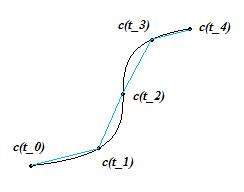
\includegraphics[scale=0.4]{images/cuasi_geodesic.jpg}
            \end{center}
        \end{figure}
        \pause
        \item Formar triángulos con cuasi-geodésicas.
        \begin{figure}
            \begin{center}
                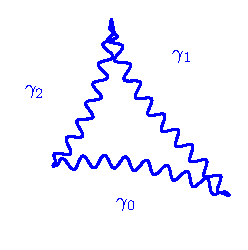
\includegraphics[scale=0.8]{images/cuasi_geodesic_triangle.pdf}
            \end{center}
        \end{figure}
        \pause
        \item Lo mismo que en hiperbolicidad ahora con cuasi-geodésicas. Esto será llamado \textbf{quasi-hiperbolicidad}.
    \end{itemize}
\end{frame}

\begin{frame}{Hiperbolicidad es invariante cuasi-isométrico}
    \begin{figure}
        \begin{center}
            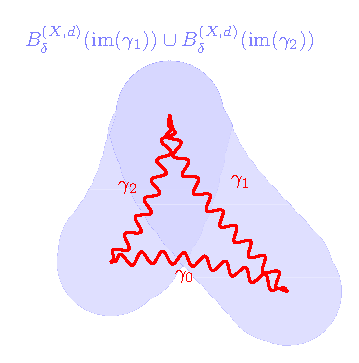
\includegraphics[scale=1.1]{images/delta_slim_qg.pdf}
        \end{center}
        \caption{Triángulo cuasi-geodésico  y $B_\delta^{(X,d)}$}
    \end{figure}
\end{frame}

\begin{frame}{Hiperbolicidad es invariante cuasi-isométrico}
    \begin{center}
        \Large \textit{¿El triángulo cuasi-geodésico anterior es $\delta$-delgado?}
        \pause

        \hfill\break

        Sí
    \end{center}    
\end{frame}

\begin{frame}{Hiperbolicidad es invariante cuasi-isométrico}
    \begin{exa}
        Todos los espacios métricos de diámetro finito son cuasi-hiperbólicos.
    \end{exa}

    \pause

    \begin{center}
        En general resultará muy complicado probar que un espacio es cuasi-hiperbólico.
    \end{center}

\end{frame}

\begin{frame}{Hiperbolicidad es invariante cuasi-isométrico}
    \begin{theor}[\textbf{Hiperbolicidad y cuasi-hiperbolicidad}]
        Sea $(X,d)$ un espacio métrico geodésico. Entonces $(X,d)$ es hiperbólico si y sólo si es cuasi-hiperbólico.
    \end{theor}
\end{frame}

\begin{frame}{Hiperbolicidad es invariante cuasi-isométrico}
    \begin{figure}
        \begin{center}
            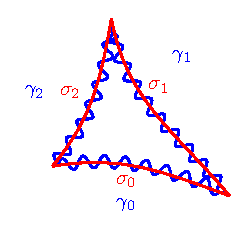
\includegraphics[scale=1.2]{images/approx_geo_cuasi.pdf}
        \end{center}
        \caption{Aproximación del triángulo cuasi-geodésico $\Delta=(\gamma_0,\gamma_1,\gamma_2)$ por el triángulo geodésico $\Delta'=(\sigma_0,\sigma_1,\sigma_2)$.}
    \end{figure}
\end{frame}

\begin{frame}{Hiperbolicidad es invariante cuasi-isométrico}
    \begin{theor}[\textbf{Invariancia cuasi-isométrica de la cuasi-hiperbolicidad}]
        Sean $(X,d)$ y $(Y,\rho)$ espacios métricos. Si $(X,d)$ y $(Y,\rho)$ son cuasi-isométricos, entonces $(X,d)$ es cuasi-hiperbólico si y sólo si $(Y,\rho)$ es cuasi-hiperbólico. 
    \end{theor}

    \pause

    \begin{cor}[\textbf{Invariancia cuasi-isométrica de la hiperbolicidad}]
        Sean $(X,d)$ y $(Y,\rho)$ espacios métricos. Si $(X,d)$ y $(Y,\rho)$ son geodésicos y cuasi-isométricos, entonces $(X,d)$ es hiperbólico si y sólo si $(Y,\rho)$ es hiperbólico. 
    \end{cor}
\end{frame}

\begin{frame}{Hiperbolicidad es invariante cuasi-isométrico}
    \begin{center}
        \Large\textit{¿Y para qué sirve la hiperbolicidad?}
    \end{center}
\end{frame}

\subsection{Grupos Hiperbólicos}

\begin{frame}
    \begin{center}
        \Large Grupos Hiperbólicos
    \end{center}
    \begin{figure}
        \begin{center}
            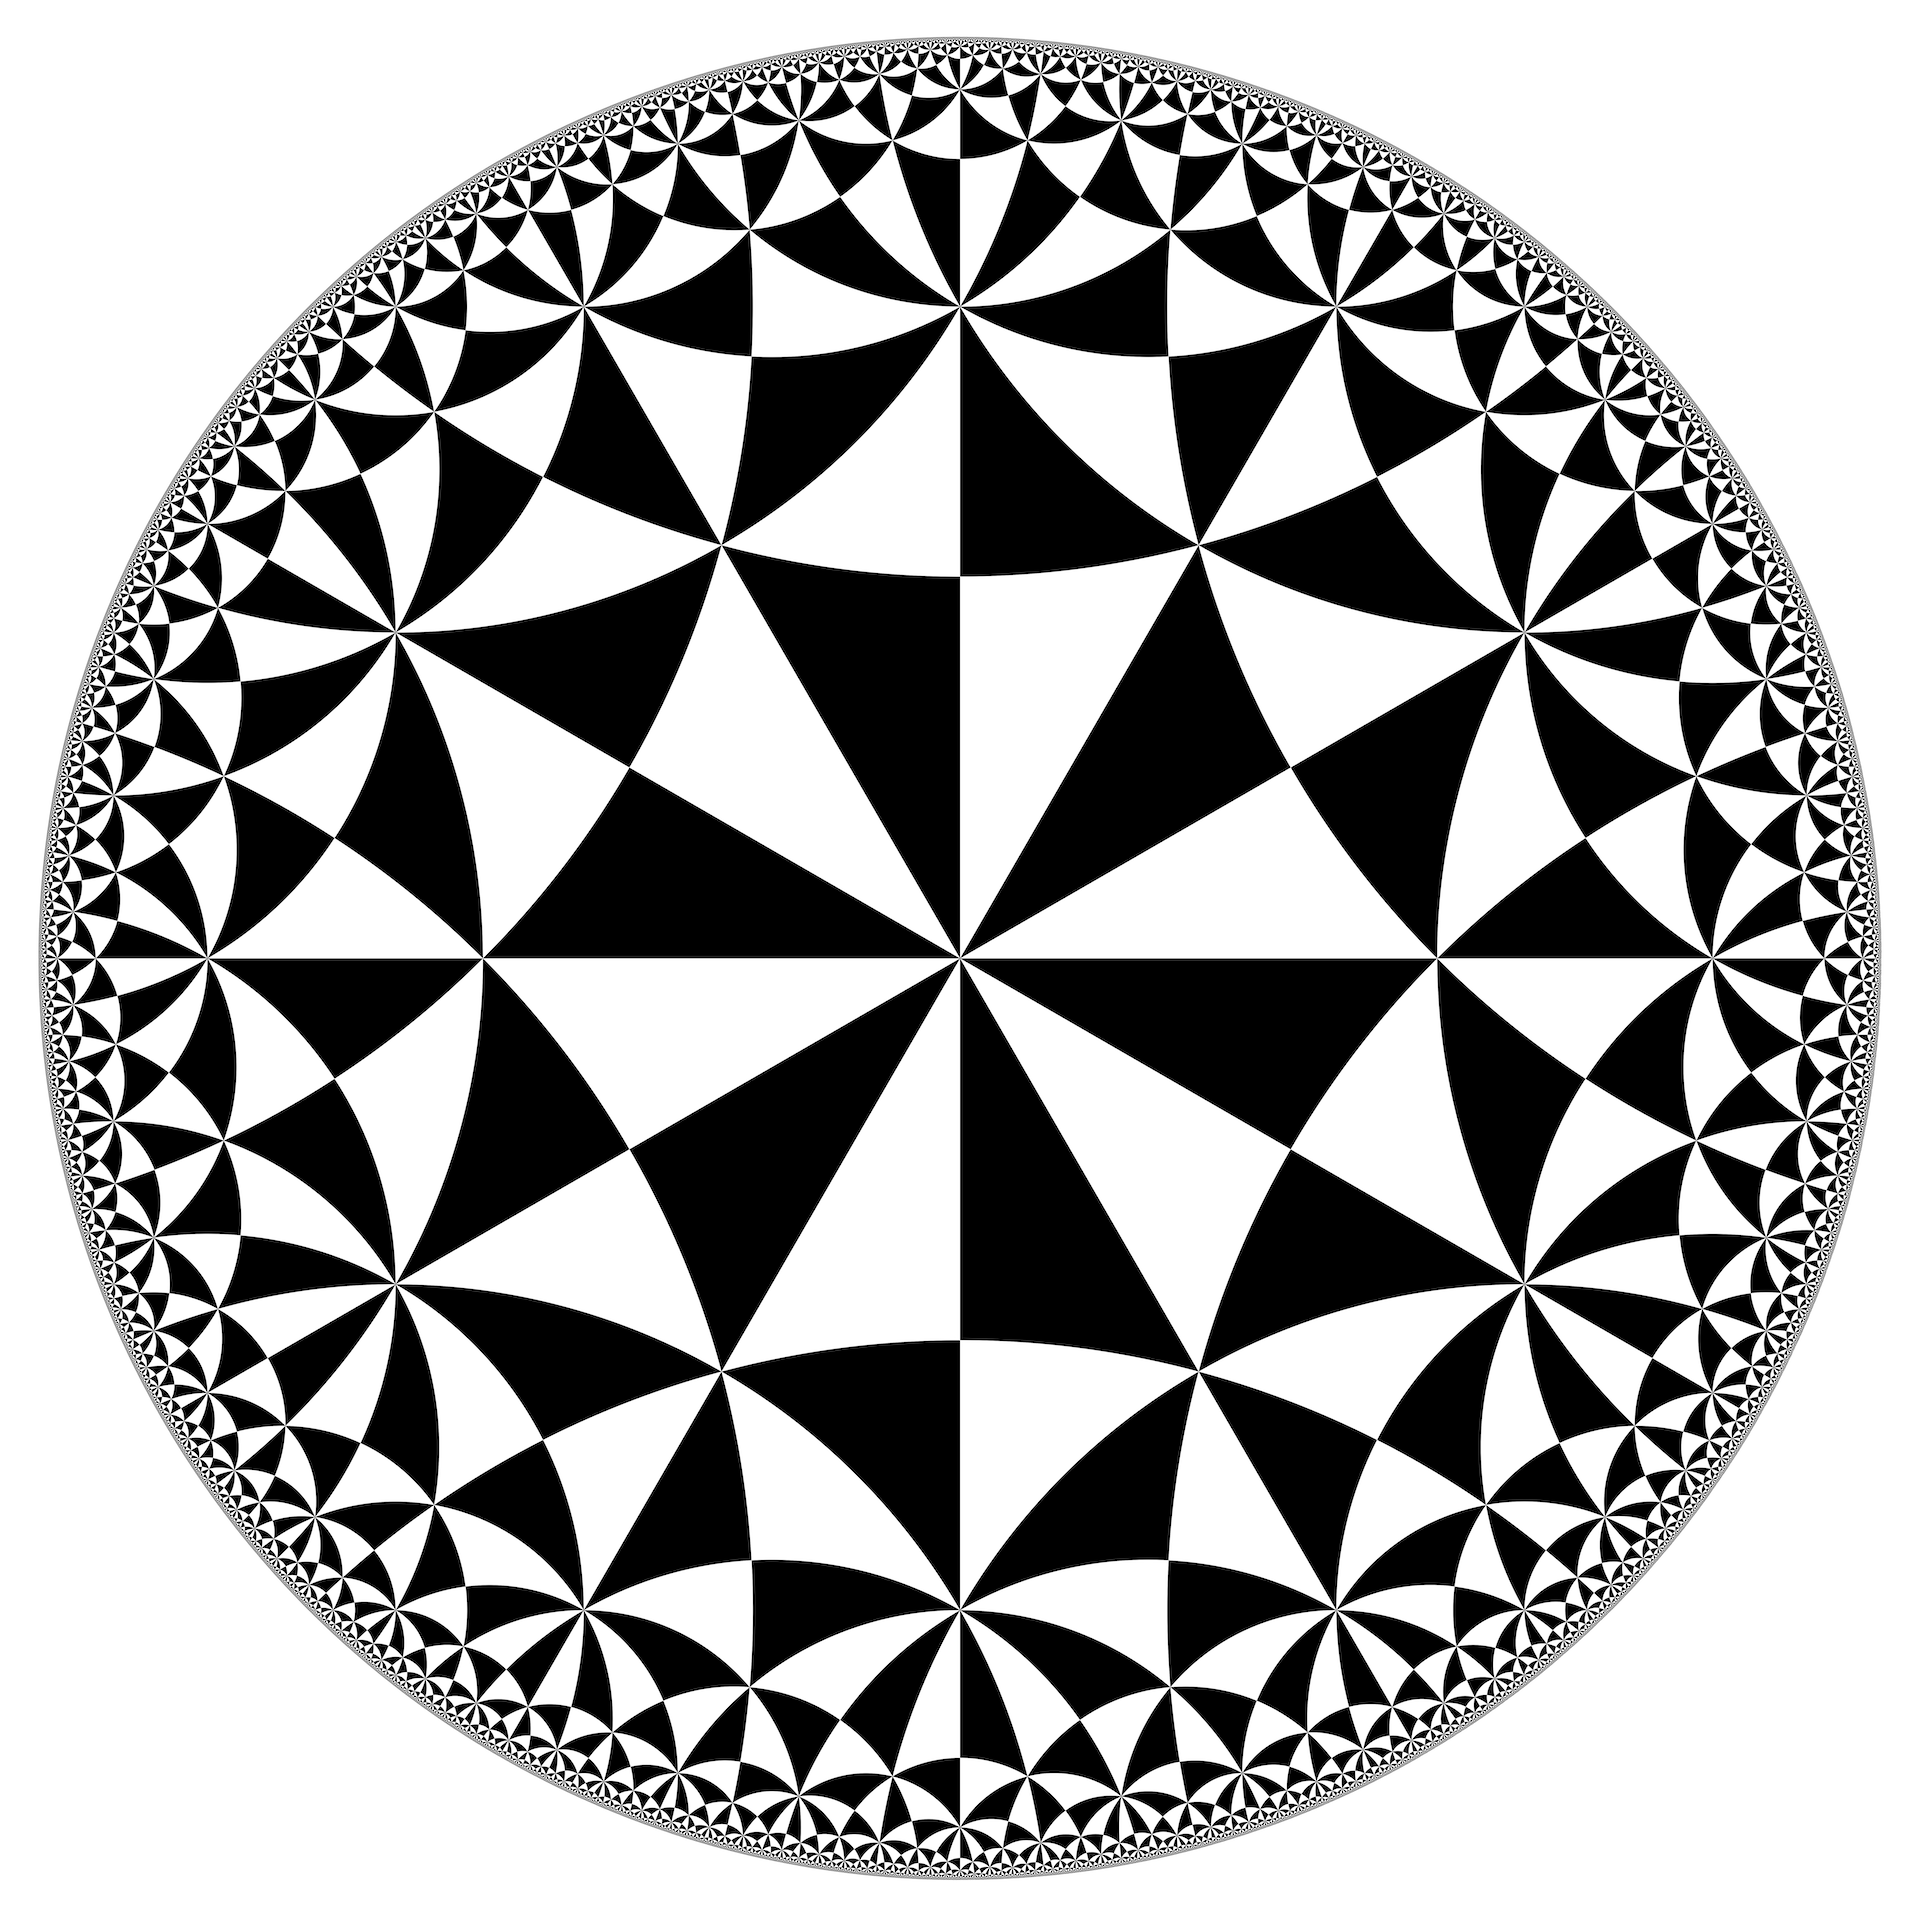
\includegraphics[scale=0.1]{images/disc_tiling.png}
        \end{center}
    \end{figure}
\end{frame}

\begin{frame}{Grupos Hiperbólicos}
    Podemos extender la noción de hiperbolicidad a grupos:

    \begin{mydef}[\textbf{Grupos hiperbólicos}]
        Un grupo finitamente generado $G$ es \textbf{hiperbólico} si para algún conjunto generador $S$ de $G$ se tiene que la gráfica de Caley $\Cay{G,S}$ es cuasi-hiperbólica.
    \end{mydef}
\end{frame}

\begin{frame}{Grupos Hiperbólicos}
    \begin{center}
        \Large Gráfica de Caley:
    \end{center}
    \begin{itemize}
        \item Asociar una gráfica a un grupo.
        \item Un grupo puede tener varias gráficas de Caley (dependiendo del conjunto generador).
        \item Es invariante cuasi-isométrico
        \item Hiperbolicidad bien definida por ser invariante quasi-isométrico.
    \end{itemize}

    \pause

    \begin{figure}
        \begin{center}
            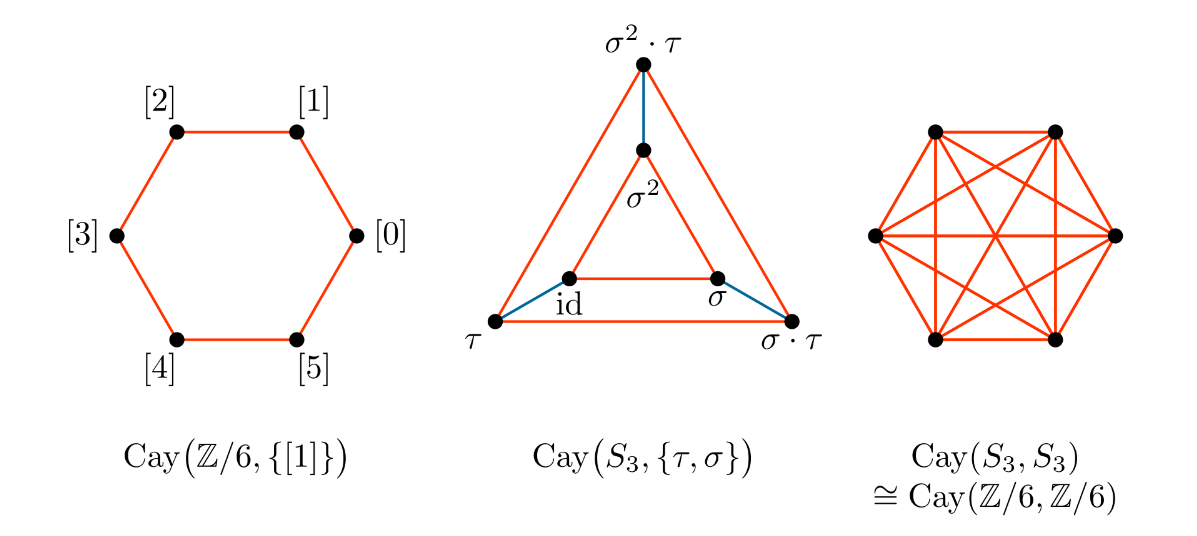
\includegraphics[scale=0.23]{images/Cayley_Graphs.png}
        \end{center}
    \end{figure}
    
\end{frame}

\begin{frame}{Grupos Hiperbólicos}
    \begin{propo}[\textbf{Hiperbolicidad es un invariante cuasi-isométrico}]
        Sean $G$ y $H$ grupos finitamente generados.  Si $G$ y $H$ son cuasi-isométricos, entonces $G$ es hiperbólico si y sólo si $H$ es hiperbólico.
    \end{propo}
\end{frame}

\begin{frame}{Grupos Hiperbólicos}

    \begin{center}
        \begin{tabular}{c | p{2.5cm}  p{2.5cm}  p{2.5cm}}
            Grupo: & $F$ Finito & $\bbm{Z}$ & $\bbm{Z}^2$ \\
              &  &  \\
            \pause Hiperbólico: & Sí & Sí & No \\
            &  &  \\
             \pause  & $\Cay{F,S}$ tiene diámetro finito & Cuasi-isométrico a $\bbm{R}$ & Cuasi-isométrico a $\bbm{R}^2$ \\
        \end{tabular}
    \end{center}

\end{frame}

\begin{frame}{Grupos Hiperbólicos}
    \begin{center}
        \Large \textit{¿De qué nos sirve generalizar esta noción a grupos?}
    \end{center}
\end{frame}

\subsection{El problema de la palabra en Grupos Hiperbólicos}

\begin{frame}
    \begin{center}
        \Large El problema de la palabra en Grupos Hiperbólicos
    \end{center}

\end{frame}

\begin{frame}{El problema de la palabra en Grupos Hiperbólicos}
    \begin{mydef}
        Sea $\gen{S|R}$ una presentación finita de un grupo. Decimos que \textbf{el problema de la palabra es soluble para la presentación $\gen{S|R}$}, si existe un algoritmo que determine en tiempo finito si una palabra de $(S\cup S^{-1})^*$ es elemento trivial de $\gen{S|R}$ o no.
    \end{mydef}
\end{frame}



%%%% ELIMINAR
\begin{frame}{El problema de la palabra en Grupos Hiperbólicos}
    \begin{exa}
        La presentación $F_2=\gen{x,y|\emptyset}$ tiene problema de la palabra soluble\pause, al igual que $\bbm{Z}^2\cong\gen{x,y|xyx^{-1}y^{-1}}$.
    \end{exa}
\end{frame}

\begin{frame}{El problema de la palabra en Grupos Hiperbólicos}
    Por ejemplo, Donald Collins encontró en 1986 que el grupo:
    
    \pause
    
    \begin{figure}
        \begin{center}
            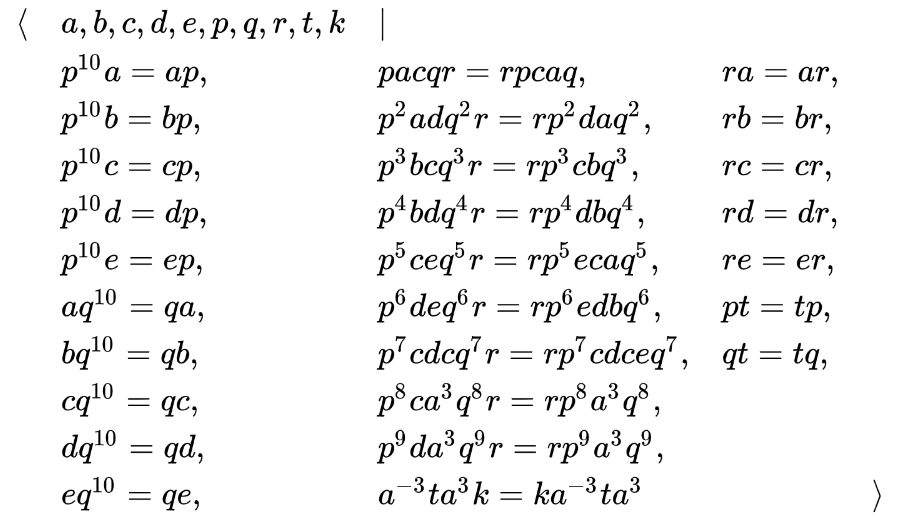
\includegraphics[scale=0.35]{images/no_soluble_word_problem.png}
        \end{center}
    \end{figure}
    
    \pause

    no tiene problema de la palabra soluble.
\end{frame}

\begin{frame}{El problema de la palabra en Grupos Hiperbólicos}

    \begin{center}
        \textit{¿Cómo garantizar solubilidad de problema de la palabra?}
    \end{center}

    \pause

    \begin{center}
        \textbf{Presentaciones de Dehn}
    \end{center}

    \pause

    Su definición da un algoritmo que hace lo siguiente:
    \begin{itemize}
        \item Nos dice como simplificar palabras.
        \item Acorta palabras.
        \item Caracteriza a los elementos neutros.
    \end{itemize}

    \pause

    \begin{center}
        Presentación de Dehn resuelven problema de la palabra.
    \end{center}

\end{frame}

\begin{frame}{El problema de la palabra en Grupos Hiperbólicos}
    \begin{propo}[\textbf{Algoritmo de Dehn}]
        Si $\gen{S|R}$ es una presentación de Dehn, entonces el problema de la palabra es soluble para $\gen{S|R}$.
    \end{propo}
\end{frame}

\begin{frame}{El problema de la palabra en Grupos Hiperbólicos}
    \begin{exa}
        La presentación:
        \begin{equation*}
            \gen{x,y|xx^{-1}e,yy^{-1}e,x^{-1}xe,y^{-1}ye}
        \end{equation*}
        es una presentacion de Dehn del grupo libre de rango 2.
    \end{exa}

    \pause

    \begin{exa}
        La presentación:
        \begin{equation*}
            \gen{x,y|[x,y]}
        \end{equation*}
        no es una presentación de Dehn de $\bbm{Z}^2$.
    \end{exa}
\end{frame}

\begin{frame}{El problema de la palabra en Grupos Hiperbólicos}
    \begin{theor}[\textbf{Presentaciones de Dehn en grupos hiperbólicos}]
        Sea $G$ un grupo hiperbólico y $S$ un conjunto generador finito de $G$. Entonces existe un conjunto finito $R\subseteq(S\cup S^{-1})^*$ tal que $\gen{S|R}$ es una presentación de Dehn y $G\cong\gen{S|R}$.
    \end{theor}
\end{frame}

\begin{frame}{El problema de la palabra en Grupos Hiperbólicos}
    \begin{cor}[\textbf{Grupos hiperbólicos tienen problema de la palabra soluble}]
        Sea $G$ grupo hiperbólico y $S\subseteq G$ un conjunto generador finito. Entonces existe una presentación finita $\gen{S|R}$ de $G$ tal que el problema de la palabra es soluble.
    \end{cor}

    \pause

    \textbf{Idea:} Atajos en ciclos dentro de grupos \textit{hiperbólicos}. Esto se logra con la acotación de triángulos que nos da la hiperbolicidad.

    \pause

    \begin{center}
        \textbf{Conclusión}: Todo grupo hiperbólico finitamente generado tiene problema de la palabra soluble.
    \end{center}
\end{frame}

\begin{frame}{El problema de la palabra en Grupos Hiperbólicos}
    \begin{center}
        \Large Grupos Fundamentales de Superficies
    \end{center}
    
    \normalsize
    
    \pause
    
    \begin{itemize}
        \item $S_g$ superficie de Riemann de género $g$.
        \item Si $g\geq 2$ entonces su cubriente universal es $\cf{p}{\bbm{H}^2}{S_g}$ (recordar Uniformización de Riemann).
        \item Se tiene:
        \begin{equation*}
            \textup{Deck}(p)=\pi_1(S_g)
        \end{equation*}
        \item Para este caso, si $f\in\textup{Deck}(p)$, entonces $f\in\Isom{\bbm{H}^2}\cong\PSL{2,\bbm{R}}$. Luego:
        \begin{equation*}
            \pi_1(S_g)<\PSL{2,\bbm{R}}
        \end{equation*}
        \pause
        \item $\pi_1(S_g)$ actúa por isometrías en $\bbm{H}^2$:
        \begin{equation*}
            (f,z)\mapsto f\cdot z= f(z)
        \end{equation*}
        cumple Svarc-Milnor.
    \end{itemize}

    \pause

    \begin{equation*}
        \pi_1(S_g)\qisom \bbm{H}^2
    \end{equation*}

    \begin{center}
        \textbf{Conclusión}: Grupos de superficies son hiperbólicos y finitamente generados, luego son finitamente presentados con problema de la palabra soluble.
    \end{center}

\end{frame}

\begin{frame}{El problema de la palabra en Grupos Hiperbólicos}
    \begin{center}
        \Large \textbf{Conclusión}: Grupos de superficies son hiperbólicos y finitamente generados, luego son finitamente presentados con problema de la palabra soluble.
    \end{center}
\end{frame}

\begin{frame}{El problema de la palabra en Grupos Hiperbólicos}
    \begin{center}
        \Huge FIN
    \end{center}

    \pause

    \begin{center}
        Gracias a Néstor, Porfirio, Rita...
    \end{center}

    \pause

    \begin{center}
        y gracias a mis compañeros de equipo: Juan, Alexia, Luis y Tadeo.
    \end{center}
    
\end{frame}

\begin{frame}{Referencias}
    \footnotesize
    \bibliography{reference.bib}
    \bibliographystyle{apalike}
    \nocite{*}
\end{frame}

\end{document}